% !TEX root = ../my-thesis.tex
%
\chapter{État de l'art}

% TODO : S'assurer que les différentes catégories scientifiques sont là
% TODO : Vérifier qu'il y a bien une justification vers un choix de progression et des parties dé-corélées sans fil conducteur.

\cleanchapterquote{Un petit chapitre pour le doctorant, un grand chapitre pour l'humanité}{Doctorant anonyme}{(Citation temporaire)}

\section{Segmentation}
\label{sec:EA:segmentation}

% Porte d'entrée par la visualisation de données

Après l'acquisition des images provenant des systèmes d'IRM et de Tomodensitométrie, se pose la question de la visualisation des données. En effet, les images obtenues sont des matrices 3D et une visualisation 3D naïve ne permet de discerner que l'enveloppe extérieure d'un volume. Parmi les techniques de visualisation, la plus simple et la moins coûteuse, revient à considérer le volume 3D comme une suite de coupes 2D. On peut ainsi visualiser la totalité des tissus d'un volume de manière itérative. Cette méthode oblige cependant les médecins à une gymnastique mentale pour reconstituer, dans leur esprit, l'organe 3D étudié. Une autre méthode consiste à visualiser les objets les plus saillants de l'image. La technique la plus utilisée, la MIP (maximum intensity projection), consiste à lancer pour chaque pixels d'un plan $p_i$, un rayon traversant le volume de donnée. L'intensité maximale des voxels le long de ce rayon est ensuite assignée à $p_i$. Cette méthode à l'avantage de faire ressortir les éléments les plus intenses de l'image et convient particulièrement à des structures mis en valeur par un agent de contraste. Elle est aussi très simple à implémenter et est peu coûteuse en ressources de calcul. Cependant, cette méthode fait perdre toute perception de profondeur, à cause de la projection, ce qui peut perturber l'analyse des structures. Ce dernier désavantage peut toutefois être contourné par l'utilisation d'une MIP dans une scène 3D contenant le volume 3D de l'image et une caméra. La projection s'effectuant alors sur le plan de la caméra et il est possible de déplacer l'observateur autour du volume qui permet grâce au mouvement de rétablir implicitement cette information de profondeur. L'utilisation de la MIP pour l'étude d'un organe, peut tout de fois être parasité par des organes adjacents plus intenses, comme par exemple les os de la cage thoracique.

A noter que ces deux méthodes ne sont pas invasives, dans le sens où aucune transformation n'est appliquée à l'image originale.

\begin{figure}
  \centering
  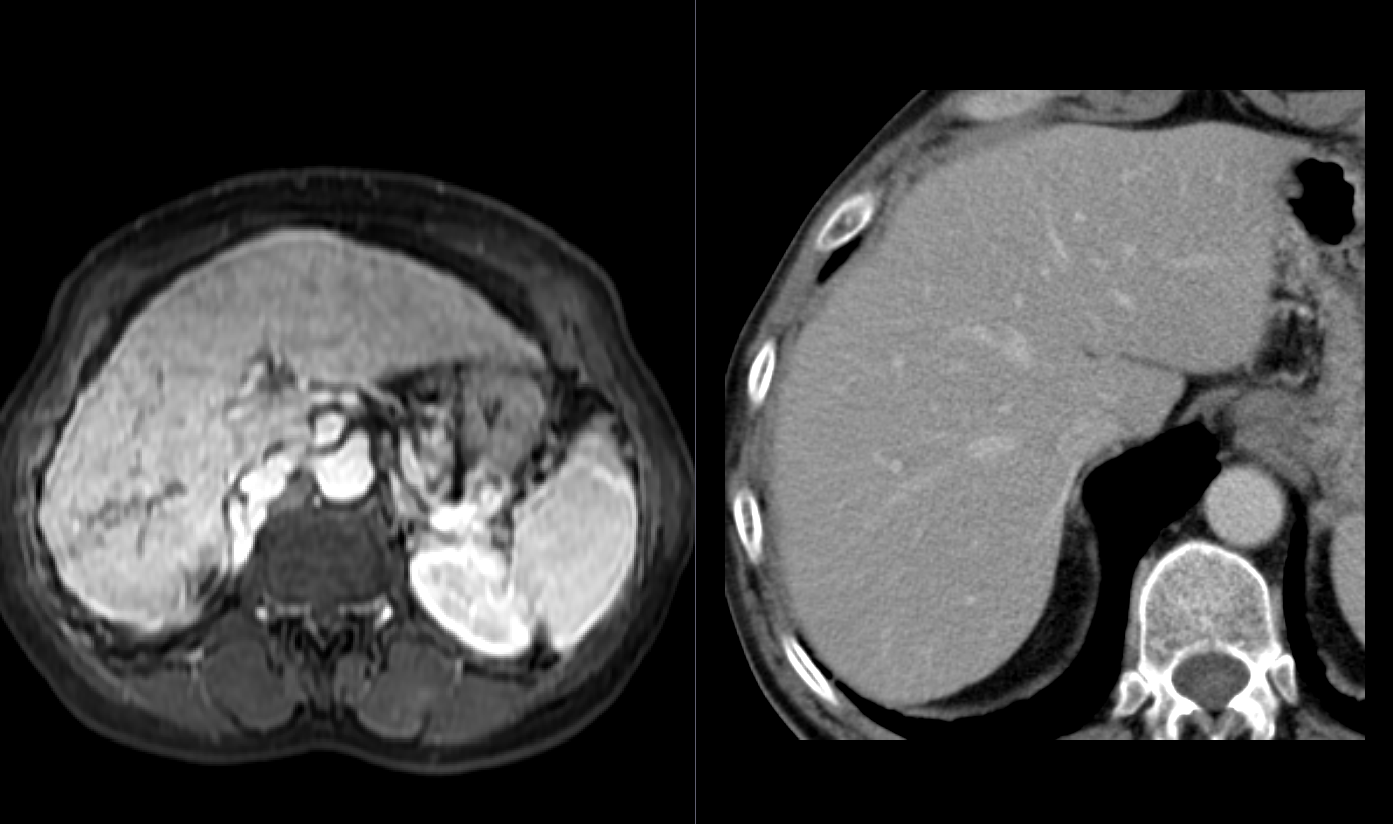
\includegraphics[height=5cm]{Images/2D_view.png}
  \label{fig:visualisation en coupe}
  \caption{visualisation en coupe, à gauche IRM, à droite tomodensitométrie}
\end{figure}

\begin{figure}
  \centering
  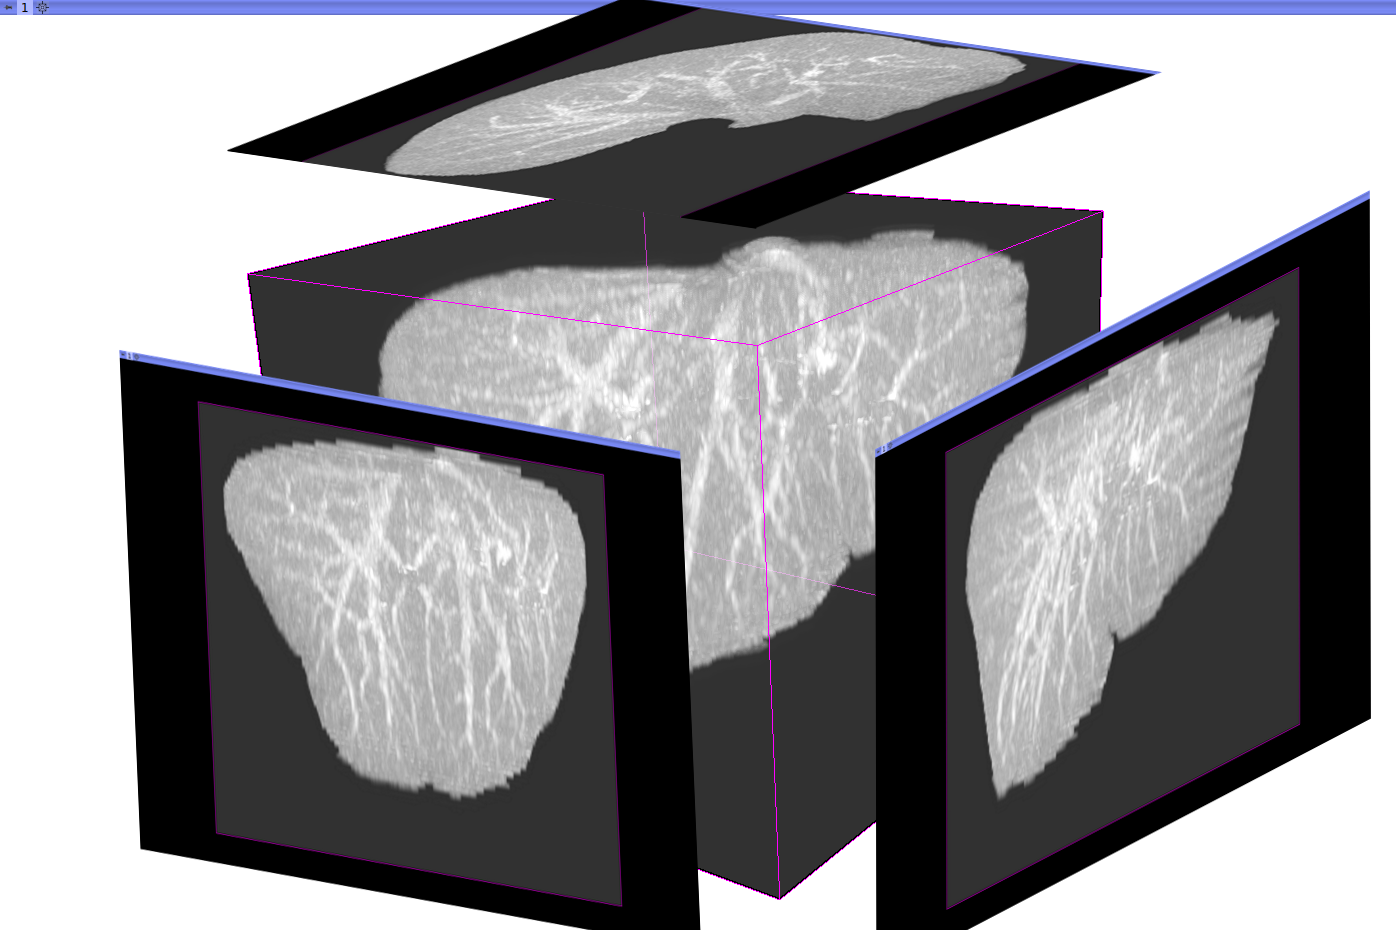
\includegraphics[height=5cm]{Images/3D_mip_montage.png}
  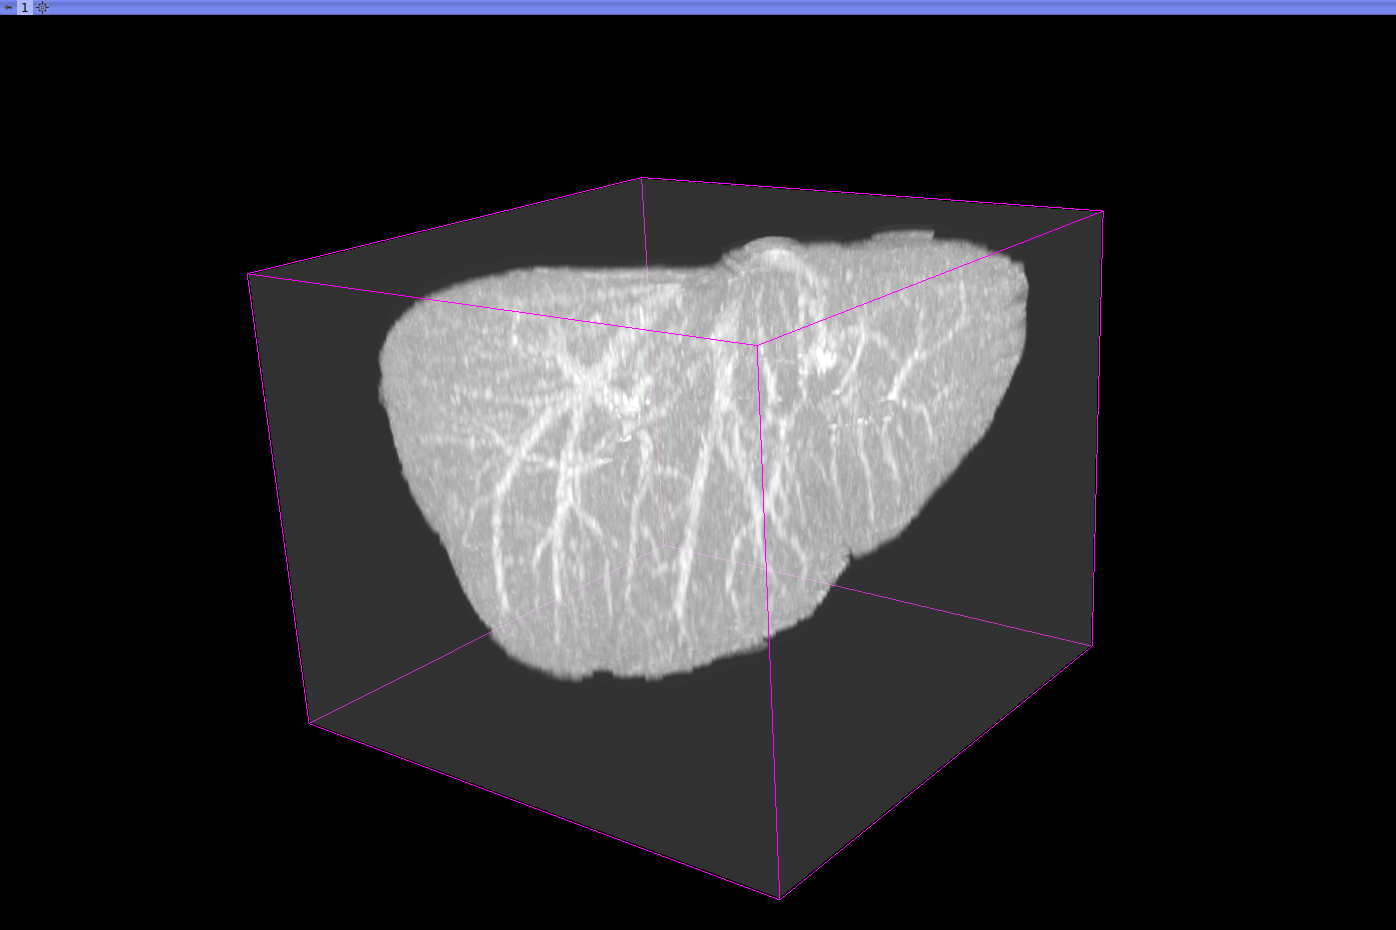
\includegraphics[height=5cm]{Images/3D_mip.png}
  \label{fig:visualisation MIP}
  \caption{Maximaly intensity projection (mip). L'intensité maximale est rétro-projeté le long du rayon sur le plan d'origine. La MIP peut s'effectuer en utilisant les bords de l'image, où le plan de la caméra dans une scène 3D}
\end{figure}

Bien que la vue en coupes 2D et la MIP offrent une visualisation convenable dans de nombreux cas, celles-ci peuvent se révéler insuffisante pour la représentation de structures complexes ou pour des tâches de mesures volumétriques. Dans ce cas, il est nécessaire d'extraire les structures d'intérêts de l'information superflux qui les entourent. C'est ce processus d'extraction que l'on nomme segmentation.

Un état de l'art des méthodes de segmentation s'est avéré nécessaire afin de choisir les outils pour l'extraction de vaisseaux hépatiques. L'objectif initial était de trouver des méthodes qui pouvaient répondre aux challenges de l'IRM du foie, c'est à dire la détection de petits vaisseaux dans un environnement faiblement contrasté, bruité avec présence potentielle d'autres structures (tumeurs). La littérature concernant la segmentation des vaisseaux hépatiques surtout en 3 dimensions est plutôt minoritaire dans la littérature. Il a donc fallu étendre cette étude aux méthodes 2D et 3D dans d'autres modalités et d'autres organes.

\subsection{Segmentation classique}
\label{sec:EA:segmentation_classique}
% Etat de l'art de la segmentation hiérarchisée par problématique
% contraste
% formea
% 
L'automatisation de la segmentation pour les images médicales est une tâche complexe. Elle doit répondre à des problématiques variées, provenant à la fois des conditions d'acquisition de l'image \ref{sec:contexte:images}, de forme de l'organe et de l'extraction d'éléments sémantiques haut niveau. Ces contraintes peuvent mener à l'élaboration de chaînes de traitements proposant un nombre d'étapes importants. Ainsi, Marcan \cite{Marcan2014_vessel_seg} propose un pipeline de segmentation en 16 étapes mélangeant, filtrage du bruit, sélection des éléments pertinents par masques et analyses des composantes connexes pour la segmentation des vaisseaux du foie. Goceri \cite{Goceri2017_vessel} propose une méthode en 14 étapes alliant partions en régions d'intérêts et étirement du contraste (contrast stretching) afin de différencier vaisseaux hépatiques des tissus du foie.

Une taxonomie précise des méthodes de segmentation est difficile à établir tant les publications présentent différentes combinaisons de briques algorithmiques. Lesage \cite{Lesage2009_review} propose une décomposition des étapes de segmentation sous la forme de 3 grands thèmes : Les modèles d'intensités et modèles géométriques, les descripteurs d'images et les schéma d'extractions. Les modèles constituent l'ensemble des hypothèses permettant d'identifier l'objet à segmenter. Les descripteurs reposent sur des caractéristiques spécifiques de l'image qui permettent de mesurer l'écart de similarité entre les données et le modèle. Enfin, le schéma d'extraction permet de choisir le seuil idéal de segmentation en fonction des caractéristiques de l'image et du/des modèle(s) choisi(s).

Dans cette partie, nous explicitons les briques algorithmiques classiquement utilisées pour la segmentation des vaisseaux. Nous prenons comme parti pris d'explorer le pipeline à l'envers, c'est à dire, de présenter les schémas d'extractions courants, puis les descripteurs communément utilisées pour finir par les modèles de représentations. Nous pourrons ainsi amener progressivement le rehaussement de vaisseaux qui se trouve à cheval entre les deux dernières catégories.

\subsubsection{Schéma d'extraction}

Une segmentation est avant tout une méthode permettant de classifier si un pixel appartient à un objet d'intérêt. Les schémas d'extractions proposent un ensemble de cadres pour automatiser ce choix.

\paragraph{Courbes de niveaux}
La méthode des courbes de niveau (level set) permet à l'origine de simuler la propagation d'une onde ou d'un fluide dans un milieu. Appliquée à la segmentation, elle permet de faire s'étendre en fonction du temps un contour jusqu'à ce qu'un critère d'arrêt soit atteint. Ce critère d'arrêt est souvent exprimé comme une énergie à minimiser. Cette énergie peut reposer sur des modélisations des structures à segmenter, des caractéristiques de l'image ou des propriétés sur la courbure du front de propagation de l'onde.

Le suivi des pixels d'un contour évoluant avec le temps est une tâche non triviale en particulier lorsque la topologie du contour change. C'est par exemple le cas lorsqu'un contour se divise en deux contours distincts. Les levels sets permettent de contourner ce problème en définissant un contour implicite comme l'intersection de deux surfaces. La première surface correspond à l'image vue comme une carte de hauteur et la seconde courbe $\phi$ correspond aux critère de partition. La dynamique d'évolution du contour implicite est géré par l'élévation de la courbe $\phi$ en fonction du temps.

Rochery et al. \cite{rochery2006_higher_active_contour} propose une segmentation des structures linéaires discontinues grâce aux level sets d'ordre supérieur contenant une énergie de continuité et une caractérisation des discontinuités. 

\begin{figure}
  \centering
  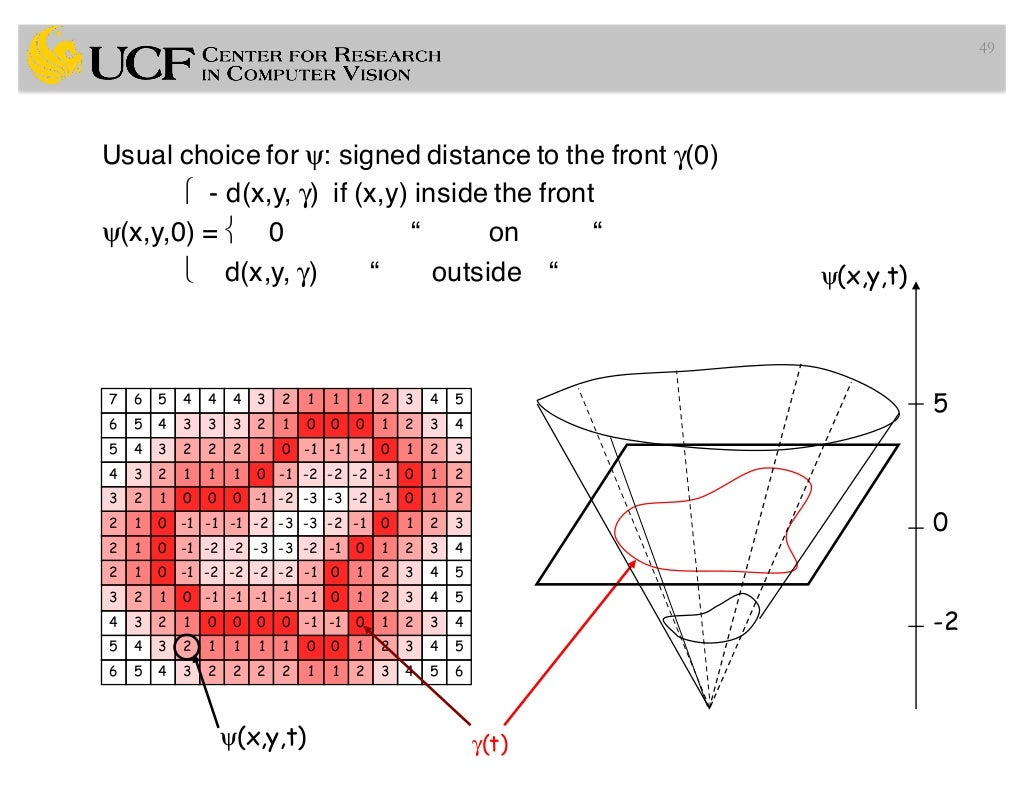
\includegraphics[height=4cm]{Images/level_set_active_contour.jpeg}
  \label{fig:Courbes de niveaux}
  \caption{Courbes de niveaux}
\end{figure}

Li \cite{Li2011_mri_level_set} utilise les levels set pour segmenter des objets malgré une intensités non homogènes, pour cela il définit un critère de classification local au voisinage des pixels afin d'estimer un champ de biais d'intensité qui est ensuite incorporé dans l'énergie de propagation. Une sous catégorie des levels set est la méthode développée par Kass et al. \cite{Kass1988_snakes} des contours actifs (aussi appelés snake). Cette méthode formule l'énergie contrôlant la propagation du contour comme la somme pondérée d'une énergie interne et d'une énergie externe à minimiser. Cette énergie a ensuite connues de nombreuses variations comme Wang et al. \cite{Wang2012_vessel_level_set} qui propose un modèle minimisant 3 énergies : une énergie basée courbure, une énergie basé sur les gradients d'intensité et une énergie basée sur un modèle cylindrique. Zeng \cite{Zeng2018_liver_hybrid_active_contour_region_growing} utilise les de contour actifs dont le critère estime à la fois la cohérence entre les régions délimités par le contour et une cartographie des contours construite sur le gradient.

\paragraph{Graph cut}

Une image peut-être représentée sous la forme d'un graphe. Dans ce graphe, les noeuds sont les pixels et les arêtes encodent une relation de similarité entre les pixels. Cette relation peut être spatiale où plus complexe. Dans ce contexte, segmenter un objet ou une région revient à trouver la coupure qui maximise la vraisemblance à l'intérieur de chaque partition et minimise la vraisemblance entre deux partitions relativement à un critère.

Zeng \cite{Zeng2017_liver_oof_graph_cut} propose un raffinement d'une segmentation initiale par graph cut, en utilisant un critère de région basé sur la vraisemblance logarithmique (negative log likelyhood) et un critère de bordure basé sur le flux (voir SEC. \ref{modèles ou rehaussement}).

\begin{figure}
  \centering
  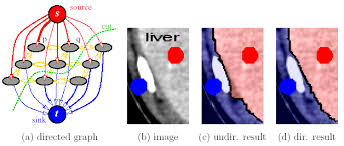
\includegraphics[height=5cm]{Images/graph_cut.jpeg}
  \label{fig:Graph cut}
  \caption{Graph cut, le graph cut nécessite des graines afin de définir les deux régions à raffiner}
\end{figure}

\paragraph{Ensembles flous}

Le choix d'une délimitation entre fond et segmentation n'est pas toujours aisé, en particulier dans les images médicales où les bords des objets à segmenter sont assez mal définis. La théorie des ensembles floues permet de modéliser cette incertitude. Au lieu d'associer une classe binaire aux pixels, on associe à chaque pixel une probabilité d'appartenance à chaque classes définie pour l'image. Un critère flou est ensuite construit afin de définir une segmentation binaire définitive.

Radojevic et al.\cite{Radojevic2015_fuzzy_logic} utilise une application à deux classes et propose une mesure d'un ensemble flou basé sur les classes multiplicatives. Cette mesure permet de définir le degrés d'ambiguïté d'un ensemble flou servant ensuite à attribuer une classe finale aux pixels.
Zhang et al. \cite{Zhang2018_liver_fuzzy_connectedness} définit un critère de connectivité floue composé d'un critère d'adjacence floue des voxels, et un critère de similarité par rapport à la géométrie d'un vaisseau basé sur les filtres de rehaussement de vaisseaux.  

%\cite{Zhang2018_liver_fuzzy_connectedness}, Fuzzy connectedness = Fuzzy adjacency (FAD) + fuzzy affinity (FA) + fuzzy connectivity (FC).
%FAD = local similarity of a voxel pair. $\mu_{\alpha}(c,d)$ monotonic increasing function, h1=exponentielle de la moyenne centrée et h2=exponentielle de la différence centrée. $w_1$ et $w_2$ sont des pondérations tel que $w_1 + w_2 = 1$. une vesselness (Zhang) est utilisée à la place de l'intensité des vaisseaux. 
%\cite{Caponetti2014_fuzzy_morphology}

%\cite{Radojevic2015_fuzzy_logic} two class application, membership function as $\mu^v=K1-Features(P)$ and $\mu^{nv}=K2-(1-Features(P))$. measure of fuzzy set = Multiplicative class : $H_*(\mu_F) = K\sum^{n}_{i=1}g( \mu_F(x_i) )$. Fuziness degree = ambiguity of fuzzy set. defuzzy-fication end $\mu^v$ vs $\mu^{nv}$.

%\cite{Sigurosson2014_retinal_morpho_fuzzy} 

\subsubsection{Caractéristiques}

Les caractéristiques extraites de l'image permettent de fournir des descripteurs quantifiables qui peuvent être incorporés dans les schémas d'extractions vus à la section précédente.

\paragraph{Opérateurs dérivatifs}

Les caractéristiques les plus employés sont les caractéristiques différentielles. Celles-ci permettent d'étudier les variations de dynamiques dans l'image et permettent notamment d'extraire des informations géométriques locales.

Le premier descripteur différentiel est la dérivée première, aussi appelé gradient. Celui-ci peut-être calculé de différentes manières (différences finies, convolution de noyau gaussien dérivés, etc.) et fourni une information sur la variation des intensités des pixels au niveau local. Le gradient est une quantité scalaire et s'exprime comme la somme des dérivées partielles de l'image. Là où le gradient permet de quantifier les changements d'intensités, l'utilisation des dérivées partielles sous forme de champ de vecteurs gradients, permet d'obtenir une information de direction du gradient. Agam et al. \cite{Agam2005_vessel_1st_order} se sert d'un champ de vecteur régularisé afin de caractériser les vaisseaux.
 
En particulier, une représentation compacte de l'orientation de la géométrie locale autour d'un pixel est le tenseur de structure qui correspond en statistique à la matrice de co-occurence qui sert à mesurer la dispersion d'une variable aléatoire.

\begin{equation}
T(f) =
\begin{bmatrix}
t_{11} & t_{12} & t_{13} \\
t_{21} & t_{22} & t_{23} \\
t_{31} & t_{32} & t_{33} \\
\end{bmatrix}
  =
\begin{bmatrix}
{\frac{\partial t}{\partial x_1}}^2 & \frac{\partial^2 f}{\partial x_1 \partial x_2} & \frac{\partial t}{\partial x_1 \partial x_3} \\
\frac{\partial t}{\partial x_2 \partial x_1} & {\frac{\partial t}{\partial x_2}}^2 & \frac{\partial t}{\partial x_2 \partial x_3} \\
\frac{\partial t}{\partial x_3 \partial x_1} & \frac{\partial t}{\partial x_3 \partial x_2} & {\frac{\partial t}{\partial x_3}}^2 \\
\end{bmatrix}
\nonumber
\end{equation}

La dérivée seconde permet d'obtenir des informations sur la courbure local de l'image autour d'un pixel. Le laplacien, qui s'exprime comme la divergence du gradient, permet d'évaluer la ressemblance du voisinage local à une sphère. \cite{Wang2020_tensor_cut}

Tout comme pour le gradient, le laplacien est une quantité sans information de direction, on utilise la matrice des dérivées partielles secondes, la hessienne, pour encoder les informations de direction.

\paragraph{Moments}

Les moments sont des descripteurs basé sur l'intégration. Ils permettent de décrire la dispersion d'une variable aléatoire (en l'occurrence, l'intensité du voisinage d'un pixel). Les moments permettent d'obtenir des informations sur l'espérance, la variance, l'asymétrie, etc. Ceux-ci se définissent par :

\begin{equation}
  M_{qpr}= \sum_{i=0}^{N_x}\sum_{j=0}^{N_y}\sum_{k=0}^{N_z}x^py^qz^r f(x,y,z) dxdydz
\end{equation}

Avec $p,q,r$ les ordres du moment et $N_x$,$N_y$,$N_z$ la longueur de chaque axe de l'image
.

Boldak et al. \cite{boldak2003_moments} propose une segmentation des vaisseaux par tracking basé sur des moments géométriques.

\paragraph{Flux}

Adossés aux champs de vecteurs gradients et aux modèles, les caractéristiques de flux permettent d'étudier la dynamique d'intensité autour des contours d'un objet. Ces caractéristiques ont été introduites par Valilevsky \cite{Vasilevskiy2002_flux}. Ces descripteurs nécessitent un choix préalable d'un modèle géométrique d'objet à segmenter et sont relativement rigides.

\subsubsection{Modèles}

La définition de modèles pour l'objet à segmenter nous permet de mesurer la fidélité d'une région décrite par des caractéristiques.

Les modèles sont en général au nombre de trois, les modèles d'intensités, les modèles géométriques et les modèles à base d'atlas.

Les modèles d'intensités sont construits sur l'intensité prédites des structures à segmenter. Pour l'angiographie, une des hypothèse de base est que les vaisseaux ont une intensité différente des tissus qui les entourent. En particulier pour l'angiographie avec agent de contraste, les vaisseaux sont supposés clairs sur fond foncé. Dans le cas contraire,   vaisseaux foncés sur fond clair, il suffit d'inverser les niveaux de gris de l'image pour retomber sur l'hypothèse initiale.

Les modèles d'intensités peuvent être construit en amont ou iterativement au cours de la segmentation. He \cite{He2013_multi_otsu} propose une segmentation itérative par seuillage automatiques Otsu et étirement de contraste afin d'élargir peu à peu le modèle d'intensité sous jacent. Bukenya \cite{Bukenya2016_heart_otsu_top_hat_hessian}, étend cette méthode à la 3D et la renforce avec des modèles géométriques afin de faciliter la détection des petits vaisseaux de faible intensité, De la même manière BahadarKhan, utilise une méthode hybride \cite{Bahadarkhan2016_fundus_region_based_otsu}.

Parmi les méthodes qui tirent parti des modèles d'intensité, on peut citer les méthodes reposant sur la MIP, qui permettent de projeter et d'isoler les vaisseaux saillants, avant de les identifier dans le volume initial par rétro-propagation.

La méthode des K plus proches voisins permet de construire automatiquement une distribution d'intensité initiale et permet de séparer facilement les classes fond et vaisseaux et d'identifier les classes d'intensité ambiguës mélangeant vaisseaux et autres tissus. Zeng \cite{Zeng2018_auto_RG_AC_hepatic_vessels} utilise les K plus proche voisins pour servir de segmentation initiale à une croissance de région. On retrouve la même pratique chez Goceri \cite{Goceri2017_vessel}. Ces méthodes montrent leurs limites lorsque le contraste des vaisseaux est faible ou que l'image étudiée ne contient pas d'intensités homogènes pour les mêmes tissus d'un même organe, comme c'est le cas pour l'IRM.

Pour répondre à ces problématiques, des méthodes de rehaussement d'image peuvent être utilisées, tel que CLAHE,utilisé par exemple par Sigurosson \cite{Sigurosson2014_retinal_morpho_fuzzy}. Des méthodes plus poussées, permettent d'estimer les biais d'intensités comme Pavan \cite{Pavan2018_HCC_detection} pour l'imagerie du foie. Ils peuvent aussi directement être exprimés dans les schéma d'extraction, comme le level set de Li \cite{Li2011_mri_level_set}.

Les constructions itératives de modèles d'intensités sont particulièrement présents dans les techniques de tracking de vaisseaux, consistant à segmenter de proche en proche la ligne centrale des vaisseaux. Pour ces applications, les modèles Bayésien permettent de construire un modèle d'intensité à partir des voxels du chemin déjà parcouru et de prédire l'intensité attendu à la prochaine étape de l'algorithme. Ces méthodes conviennent particulièrement au tracking d'axones pour la fluoroscopie \cite{Radojevic2015_fuzzy_logic}\cite{Radojevic2017_neurons_bayesian_tracing_density}.

\begin{figure}
  \centering
  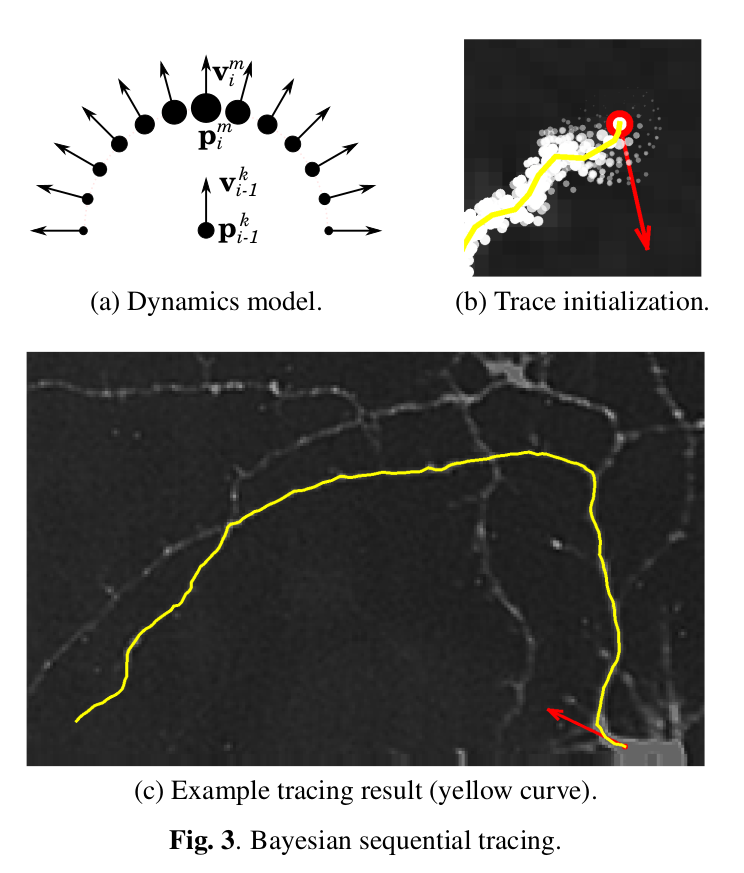
\includegraphics[height=5cm]{Images/bayesian_tracing.png}
  \label{fig:modele bayesien}
  \caption{Modèle Bayésien pour le tracking, fluoroscopy}
\end{figure}

% Modèles géométriques
Les modèles d'intensités ne prennent pas en compte la forme des objets détectés et peuvent ainsi détecter des objets de même intensités n'étant pas des vaisseaux. Par exemple, pour des vaisseaux faiblement contrastés et bruitées, la distribution d'intensité des vaisseaux risque de chevaucher la distribution du bruit.

\begin{figure}
  \centering
  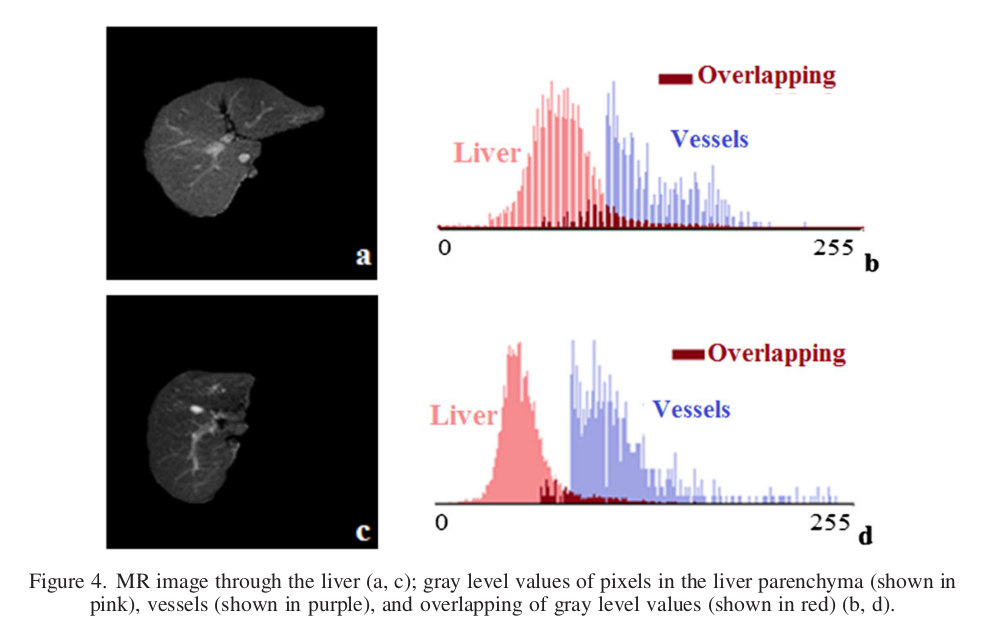
\includegraphics[height=5cm]{Images/Goceri[2016].png}
  \label{fig:overlap_vessels_tissues}
  \caption{Histogrammes d'intensité des tissus du foie, en bleu l'intensité des vaisseaux, en rouge l'intensité des tissus du foie (image placeholder, Goceri[2016] ) }
\end{figure}

Les modèles géométriques viennent compléter les modèles d'intensités. En effet, l'aspect spécifique des vaisseaux qui forment des structures curvilignes, les rendent le plus souvent très différents des autres organes.

Les modèles les plus basiques sont les modèles en forme de disques, ou sphériques pour leurs équivalents 3D \cite{Law2008_OOF}. Les modèles sphériques sont limités par le fait que les éléments sphériques et tubulaires ne sont pas dissociables. Des variantes cylindriques ont aussi été proposées dans la littérature Tyrrell \cite{Tyrrell2007_superEllipoid}, Esneault \cite{Esneault2009_moments_graph_cut}, Cetin \cite{Cetin2015_high_order}. Le modèle prédominant est le modèle tubulaire  développé dans le chapitre CH.\ref{Chap4-benchmark} Celui-ci a l'avantage d'être plus général et flexible que le modèle cylindrique.

La littérature propose aussi un ensemble de modèles déformables, sans à priori de formes. Ceux-ci nécessitent le plus souvent un point d'initialisation donné manuellement ou déterminé de manière automatique. Ces modèles sont contraints par une énergie qui définie les limites de déformation du modèle. La difficulté principale est de trouver un terme de contrainte permettant d'éviter un écoulement du modèle hors des vaisseaux. Mille et al. \cite{Mille2009_deformable} combine un critère de tubularité, un critère d'homogénéité de régions et un critère de lissage du contour. 

Enfin, une famille de modèle provenant de la morphologie mathématique modélise les vaisseaux comme un ensemble de chemins curvilinéaires.\cite{Heijmans2005_path_opening}

\begin{figure}
  \centering
  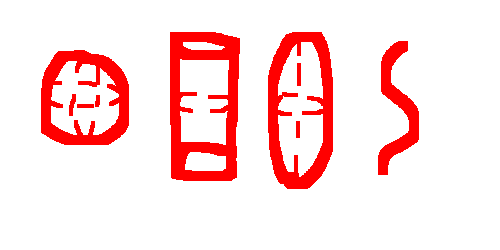
\includegraphics[height=5cm]{Images/geometricModels.png}
  \label{fig:geometricModels}
  \caption{Modèles géométriques basiques, sphère, cylindre, tubulaire et curvilinéaire}
\end{figure}

Enfin, les modèles à base d'atlas sont des modèles construits à base de mesures préalables. Ils sont construit en amont de la méthode de segmentation et représentent une connaissance ``en moyenne'' d'un modèle géométrique, d'intensité ou plus fréquemment d'une localisation dans l'espace. Les modèles d'atlas sont particulièrement adaptés à des structures rigides qui présentent peu de diversités anatomiques comme les vaisseaux du cerveau, Passat et al. \cite{passat2006_atlas}.

\subsection{Segmentation deep learning 3D}
\label{sec:EA:segmentation_deep3D}

A partir de 2015, les réseaux de neurones ont pris une place prépondérante dans la littérature de la segmentation grâce à l'apparition des modèles de réseaux profonds, de l'augmentation de la puissance de calculs et d'un nombre important de données annotées. Pour le médical cette installation se fait de manière plus lente mais assurée. La classification  modèle, caractéristiques, schéma d'extraction est plus complexe à appliquer en deep learning. Celui-ci repose sur trois éléments, l'architecture du réseau, les données utilisées associées et le critère de convergence du réseau.

% Que le médical
\subsubsection{Architecture}
% Architecture
% 1) Réseaux de neurones à convolution
% 2) Types d'entrainement, supervisé vs non supervisé
Les réseaux de neurones convolutifs ont pris une place prépondérante dans la littérature. Ces méthodes reposent sur l'apprentissage automatique de caractéristiques de l'image. Pour cela, un grand nombre d'exemples est montré au réseau qui apprend à donner la réponse attendue. Deux types d'entraînement sont principalement utilisés, l'entraînement supervisé par paires \{image d'entrée,vérité terrains\} et l'entraînement non supervisé avec des images en entrée et une énergie à minimiser, permettant de contraindre la sortie du réseau. L'erreur de classification du réseau est ensuite propagée à travers chaque couches qui le compose par rétro-propagation du gradient d'erreur.

Les réseaux convolutionels sont une représentation compactes de réseaux plus anciens, les perceptrons multi-couches. Ils ont aussi la propriété d'être invariant à la translation.
% 4) Publications milestones (AlexNet,VGG,ResNet,DenseNet,U-Net)
% 5) Variantes de Unet (Res-Unet,Vesselnet, branches multiples)

AlexNet \cite{krizhevsky2012_AlexNet} et VGG \cite{Simonyan2014_VGG} marquent le début des réseaux de convolution profonds (CNN) avec des performances remarquables pour la classification d'images couleurs. Avec la création de réseaux de plus en plus profonds, l'entraînement se révèle de plus en plus difficile à cause de la diminution croissante de l'erreur à rétro-propager au fur et à mesure des couches. Ce problème a été résolu plus tard par le modèle ResNet \cite{He2016_ResNet}, qui propose des couches résiduels permettant d'introduire une redondance de l'information. De la même manière, le modèle DenseNet \cite{Huang2017_DenseNet} propose de réutiliser des caractéristiques tout au long du réseau, alliant redondance et légèreté du réseau.

Ce sont les réseaux convolutionels complets (FCNN), en particulier l'architecture d'auto-encodeur U-Net \cite{Ronneberger2015_Unet} qui a percé dans le milieu médical en permettant de segmenter de manière précise des organes. Ce modèle propose une architecture composé d'un encoder et d'un décoder symétriques, donnant au réseau sa forme en U caractéristique. Des ``skip connections'', permettent de propager les détails de l'encoder au décoder.

Un large panel de variantes de ce réseau a été proposé dans la littérature, combinant ResNet \cite{yu2019_liver_ResUnet}, DenseNet \cite{Li2018_DenseUnet}, en utilisant plusieurs réseaux à des résolutions différentes ou en proposant des branches spécialisées.

L'entraînement d'un réseau est possible seulement si l'on est capable de définir une mesure de l'erreur produite entre la sortie d'un réseau et le résultat attendu. Cette fonction de coût, aussi appelée fonction de perte (loss function) a aussi largement été étudiée dans la littérature. Les premières fonctions de coût reposent sur la distance L2. Celle-ci a été largement remplacée par une fonction de coût empruntée de la théorie de l'information, la cross entropie. Pour la segmentation, Sudre \cite{Sudre2017_DiceLoss} propose une fonction de perte, la ``Dice loss'' basée sur le recouvrement entre la vérité terrain et la segmentation du réseau. Plusieurs métriques ont été dérivées de la Dice loss, tel que la fonction de perte de Tversky ou focale. Ces fonctions permettent de régler la sensibilité de la métrique au taux de faux positifs ou de faux négatifs. Une revue des fonctions de perte pour la segmentation est proposé par \cite{Jadon2020_survey_seg_loss}. Plus récemment des travaux ont exploré l'introduction de critères topologiques (composantes connexes) afin de limiter la fragmentation des segmentations \cite{Hu2019_topo_homo_persi},\cite{Clough2019_topo_homo_persi},\cite{Ventura2017iterative_topo}. Ces méthodes restent très coûteuses en temps.


Le nombre des données joue un rôle crucial dans la performance des réseaux de neurones. Pour l'imagerie médicale, deux problèmes se posent. Le premier concerne l'acquisition et la collecte des données. En effet, un examen médical n'est réalisé que lorsque celui-ci est jugé nécessaire. De plus, la législation concernant la collecte, le stockage et l'anonymisation des données est de plus en plus stricte depuis la RGPD.

Un second problème qui concerne particulièrement les méthodes supervisées est l'annotation des données collectées. Pour la segmentation d'images médicales, cette vérité terrain est nécessaire pour à la fois valider les modèles utilisés et faire converger les réseaux. Cependant, l'annotation est une tâche longue et fatigante qui nécessite la mobilisation d'un ou de plusieurs spécialistes.

Plusieurs méthodes permettent de contourner partiellement ce problème. La plus utilisée est l'augmentation de données, \cite{Liskowski2016_data_augmentation}. Celle-ci utilise des données existantes pour appliquer des changements d'intensités ou des déformations géométriques afin de créer artificiellement des données supplémentaires.

D'autres méthodes comptes sur l'utilisation de données partielles, ou d'annotations complètes sur une partie des données seulement \cite{Tajbakhsh2020_imperfect_datasets}. Certains auteurs ont exploré le transfert de style afin de générer des images d'une modalité grâce à des images d'autres modalités. Chartsias et al. \cite{Chartsias2017_heart_adversarial_im} propose la génération adversaire d'images IRM grâce à des images CT et un masque d'alignement des structures. Chartsias montre qu'en entraînant un réseau sur des images réelles et synthétiques, on augmente les performances d'un réseau de segmentation. Huo et al. \cite{Huo2018_adversarial} explore la génération à la fois d'une nouvelle modalité et de sa segmentation.

\subsection{Bilan sur la segmentation}

Malgré une littérature dense, il n'est pas facile de juger de l'efficacité d'une méthode de segmentation sur une autre. Cette difficulté s'illustre dans les tableaux comparatifs de l'état de l'art conduit par  Moccia et al. \cite{Moccia2018_survey}. Ils montrent un problème à plusieurs niveaux .

Premièrement, il y a disparité dans les métriques de comparaisons. Certains papier utilisent les métriques standard de classification : précision, accuracy, sensibilité, spécificité. d'autres articles utilisent des métriques de recouvrement comme le Dice ou les coefficients de corrélations de Matthew (MCC) et d'autres des opérateurs intégraux de type AUC, ROC. Les résultats de certaines méthodes sont mêmes évaluée visuellement par des experts.

Deuxièmement, il y a une disparité dans les jeux de données. Les jeux de données utilisés entre deux articles proviennent souvent de sources différentes. Le nombre d'images traités, les paramètres d'acquisition des modalités varient et les jeux de données ne sont pas toujours disponible publiquement, en particulier pour les données 3D. Cette disparité est à minimiser pour les images 2D couleurs de fond de l'oeil (fundus) qui disposent de 3 jeux de données annotés qui font référence. L'accessibilité de ces jeux de données annotés est en partie responsable du grand nombre d'articles les utilisant.

Troisièmement, il est difficile de juger des bénéfices de chaque blocs algorithmiques dans le pipeline de segmentation. Une étude ablative où chaque bloc est remplacé afin d'étudier sa performance, comme on pourrait le faire en deep learning n'est pas forcément possible. Il est donc complexe de juger si une méthode est efficace grâce à sa modélisation du problème, l'utilisation de caractéristiques ou de la pertinence de son schéma d'extraction.

Pour le deep learning, la problématique se situe au niveau des données. L'objectif d'analyser la structure 3D des images IRM hépatiques pose deux problèmes. Le premier est le manque de données annotés qui limite grandement l'utilisation de méthodes supervisées. Le second est l'usage de la 3D qui augmente de manière significative le besoin en ressource de calcul.

Afin de trouver un positionnement adéquat, nous avons choisis de nous concentrer sur une famille de filtres vasculaires couplant modèles et caractéristiques régulièrement présents en amont des chaînes de traitements. Leur position fait de ces filtres des éléments clés impactant fortement le choix des schémas d'extractions et le résultat de la segmentation finale. C'est filtres ont aussi la possibilité d'être utilisés comme données d'entrée d'un réseau de neurone. Une étude préliminaire de leurs propriétés nous paraissait donc pertinent comme premier pas vers la construction d'un algorithme de segmentation.

\section{Rehaussement}
\label{sec:EA:rehaussement}
\subsection{Introduction}
\label{sec:EA:rehaussement:introduction}

Parmi les méthodes de segmentation des vaisseaux sanguins une grande majorité utilise une étape de pré-traitement consistant à faciliter la segmentation des vaisseaux. Cette étape augmente de manière significative le contraste des vaisseaux et atténue le signal de toutes les autres structures. Ces filtres portent le nom de ``filtres de rehaussement de vaisseaux'' (vesselness filters). Ces filtres combinent des modèles d'intensités et de géométries spécifiques aux vaisseaux avec des descripteurs d'images. De par leur positionnement en amont des pipelines de segmentation, ils ont une influence directe sur le choix et les performances des schémas d'extractions.

\begin{figure}
  \centering
  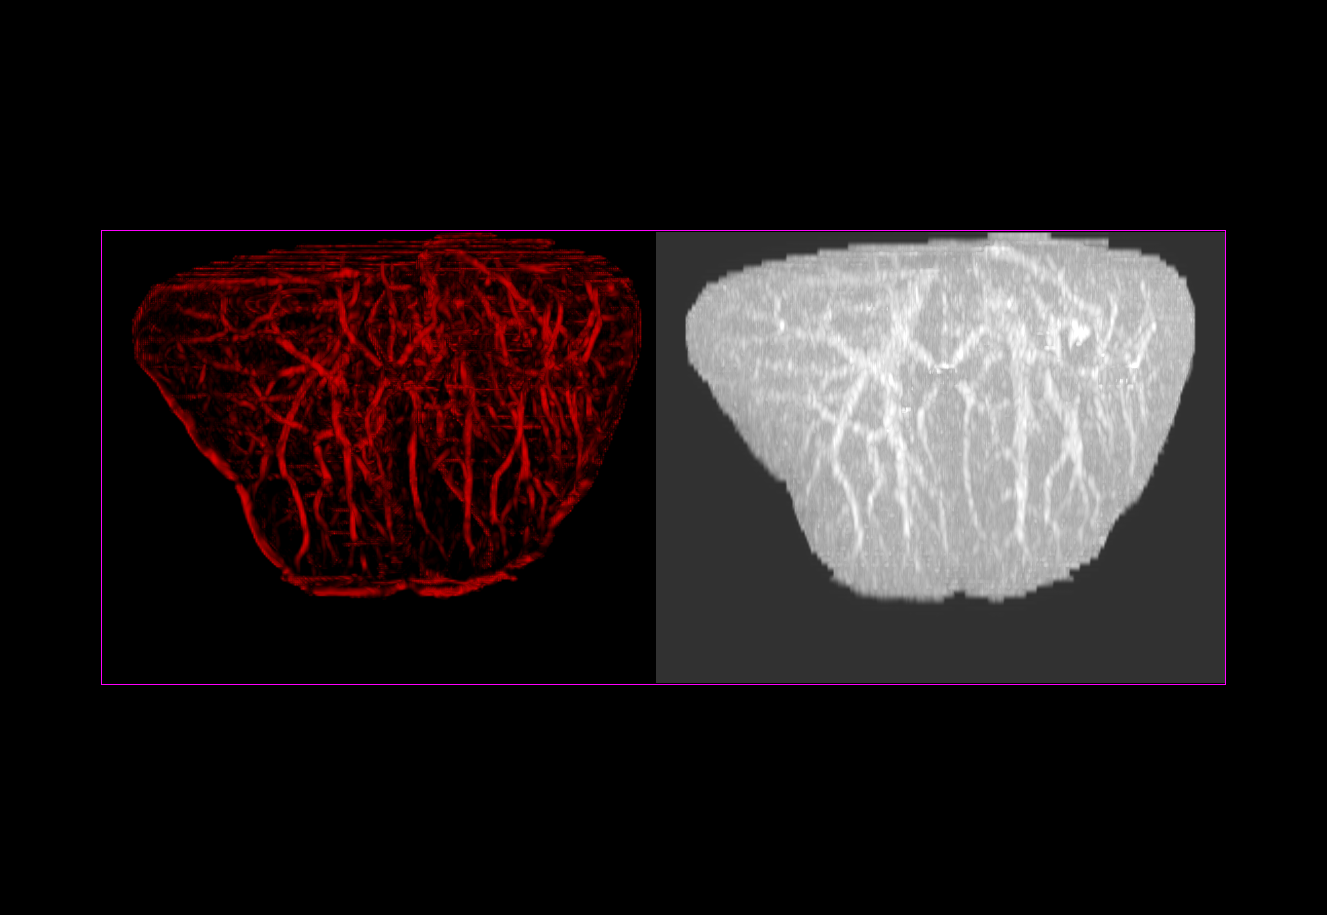
\includegraphics[height=4cm]{Images/vessels_enhancement.png}
  \label{fig:placeholder}
  \caption{Exemple de rehaussement de vaisseaux}
\end{figure}

Un filtre de rehaussement peut se baser sur plusieurs stratégies pour améliorer le signal des vaisseaux :

\begin{itemize}
\item la distribution des intensités
\item la géométrie des structures
\item la hiérarchie des structures
\end{itemize}

En effet, pour la tomodensitométrie comme pour l'IRM, certaines hypothèses physiques sont applicables aux vaisseaux.

Premièrement, pour l'angiographie avec injection d'agent de contraste, on considère que les vaisseaux ont une intensité supérieure aux tissus qui les entourent. Cette hypothèse, bien que souvent vraie, se retrouve limitée en pratique. En effet, cette hypothèse dépend des conditions liées au temps d'acquisition et de la vascularisation de l'organe étudié. Plus l'acquisition est longue et les échanges vasculaires nombreux dans l'organe, plus l'agent de contraste se diffuse dans celui-ci. Ce processus peux aller jusqu'à rendre l'organe totalement uniforme sans possibilité de différencier les tissus qui le compose. Comme discuté dans la section SEC. ~\ref{sec:contexte:images} du chapitre CH.~\ref{} l'utilisation d'agent de contrastes ne garanti pas un aspect uniforme des vaisseaux. Cet aspect varie en fonction de la concentration de l'agent de contraste dissous dans le sang. Par conséquent, plus le diamètre des vaisseaux est réduit, plus la concentration, et donc le contraste, est faible. Pour des tronçons de vaisseaux de même taille, la viscosité du sang ou la géométrie des vaisseaux peut aussi faire s'accumuler l'agent de contraste dans des régions spécifiques.

Une fois l'hypothèse d'intensité posée, on peut établir de nouvelles hypothèses sur la géométrie des vaisseaux. L'hypothèse la plus courante est d'assimiler les vaisseaux à des cylindres ou des tubes soumis à des contraintes géométriques plus ou moins relâchées. Cette hypothèse peut se montrer suffisante lorsque l'on ne considère qu'un seul tronçon de vaisseaux. En réalité, dans un réseau vasculaire, chaque tronçons peut avoir des formes et diamètres variés, et les tranches successives d'un même tronçon ne sont pas forcément homogène. De plus, les vaisseaux sont inter-connectés entre eux, formant aux jonctions des objets géométriques qui sortent du cadre des hypothèses initiales.

Enfin, on peut établir des hypothèses basées sur la hiérarchie des vaisseaux. La plupart du temps, les organes sont alimentés par un ou des vaisseaux principaux, les artères, relativement larges qui se subdivisent ensuite pour alimenter les différentes régions de l'organe. Cette subdivision prend la plupart du temps la forme d'une bifurcation, c'est à dire un vaisseaux se séparant en deux vaisseaux (pour les artères, et inversement pour les veines). Plus rarement, on peut observer des N-furcations, comme la trifurcation de la carotide. Cette division des vaisseaux est la plupart du temps accompagnée d'un changement de diamètre qui dépend du sens du flux sanguin. Dans certains organes, on peut ainsi vérifié des propriétés topologiques. Par exemple pour le foie, le réseau vasculaire porte peut être assimilé à un graphe sans cycle, voir à un arbre dont les noeuds sont les bifurcations et les arêtes les vaisseaux.

\begin{figure}
  \centering
  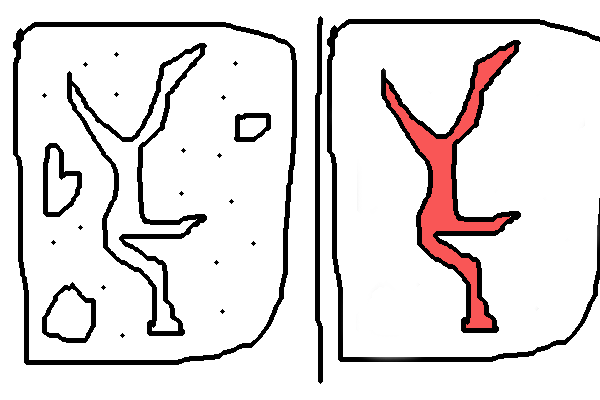
\includegraphics[height=5cm]{Images/example_enhancement.png}
  \label{fig:exemple_vesselness}
  \caption{exemple de filtre de rehaussement de vaisseaux}
\end{figure}

\section{Espace d'échelle}
\label{sec:EA:rehaussement:echelle}


La détection d'un réseau vasculaire dans sa totalité implique de détecter des vaisseaux de différentes tailles. En effet, les plus gros vaisseaux peuvent faire plusieurs dizaines de voxels de diamètres tandis que les vaisseaux les plus fins, atteignant les limites de la résolution des capteurs, peuvent  mesurer jusqu'à un voxel de diamètre. Il n'est pas envisageable de réécrire un algorithme pour chaque taille de vaisseaux, c'est pourquoi des cadres théoriques, appelés \emph{espace d'échelle} ont été formulés. Ces espaces d'échelles permettent d'établir un cadre uniforme pour sélectionner les structures d'une image à une échelle donnée. Trois espaces d'échelles sont couramment associés au rehaussement de vasculaire dans la littérature : L'espace d'échelle gaussien, l'espace d'échelle granulométrie et l'espace d'échelle de flux orienté.

\subsection{Espace Gaussien}
\label{sec:EA:rehaussement:echelle:gaussien}

% what we want to say
% why gaussian ?
% - smoothing remove lower structures without introducing new ones
% - relation between sigma and sizes
% - relation to sigma and vessels radius
Lindenberg introduit la théorie de l'espace d'échelles gaussien dans \cite{lindeberg2013_scale}. Dans cette théorie, a l'échelle la plus basse, la totalité des structures sont présentes, et les détails les plus fins sont présents. Au fur et à mesure que l'échelle augmente, les détails sont lissés pour ne laisser que les maxima locaux correspondants aux formes les plus grandes. Ainsi, l'échelle minimale correspond à l'image initiale et l'échelle maximale correspond à une image uniforme. Il a été démontré que les noyaux gaussien étaient les seuls noyaux permettant de passer d'une échelle fine à une échelle grossière sans provoquer l'apparition de nouvelles structures. De plus, un mécanisme identique a été observé dans le fonctionnement du champ visuel.

\begin{figure}
  \centering
  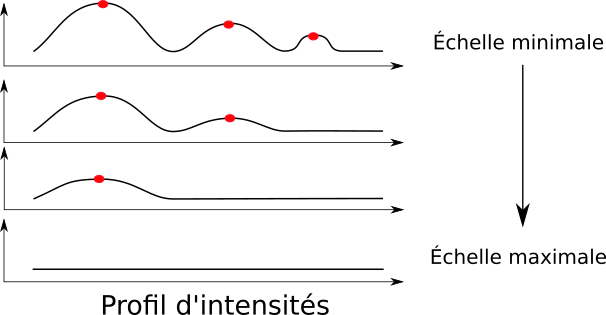
\includegraphics[height=5cm]{Images/gaussian_smoothing.png}
  \label{fig:gaussian_smoothing}
  \caption{Lissage gaussien, les structures de taille égales ou supérieures à $\sigma$ sont conservées alors que les structures de taille inférieures disparaissent}
\end{figure}

\begin{equation}
  gauss(x,y,\sigma_{x},\sigma_{y}) = \frac{1}{ \sigma\sqrt{2\pi} }exp(-\frac{x^2 + y^2 + z^2}{2(\sigma_{x}+ \sigma_{y}+ \sigma_{z}) })
\end{equation}

La sélection de l'échelle dans un espace gaussien se fait par le choix de l'écart-type $\sigma$ de la gaussienne. La plupart du temps on considère un espace d'échelle uniforme, $\sigma_x = \sigma_y = \sigma_z$. Il faut noter que pour un $\sigma$ donné, la taille des structures n'est pas supérieure ou égale à $\sigma$ mais plutôt supérieure ou égale à $\alpha\sigma$. En effet, en empruntant le formalisme des statistiques, l'intervalle de confiance, c'est-à-dire la couverture d'une distribution normale, correspond à $34.1\%$ pour $\sigma=1$, $68\%$ pour $\sigma=2$ et $99.7\%$ pour $\sigma=3$. Ainsi, pour $\sigma=1$ on détectera des objets de rayon $3\sigma$ et de diamètre $6\sigma$.  

\begin{figure}
  \centering
  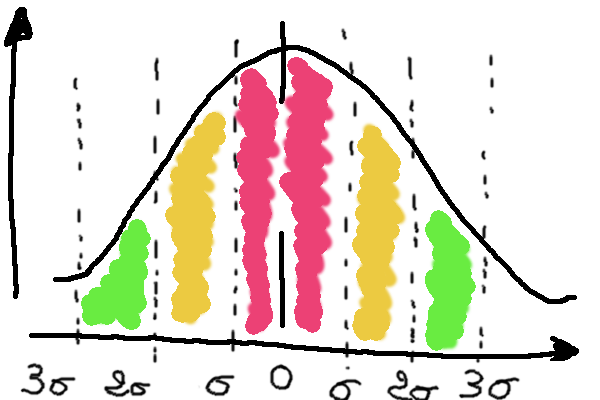
\includegraphics[height=5cm]{Images/normal_distribution_probability_coverage.png}
  \label{fig:normal_distribution_probability_coverage}
  \caption{couverture d'une distribution normale}
\end{figure}

L'espace gaussien se prête particulièrement bien à la modélisation des vaisseaux. En effet, la formulation de la gaussienne correspond bien à l'effet combiné des hypothèses de vaisseaux cylindriques et de la diminution d'intensité des vaisseaux au fur et à mesure que l'on s'éloigne de leur centre. En particulier pour un vaisseau parfait de diamètre $3\sigma$, les maxima locaux se situent le long de sa ligne centrale.

De plus, la gaussienne se prête très bien à une analyse locale de la géométrie basée sur la dérivation. Elle assure en effet les hypothèses de continuité du support de l'image et permet de combiner lissage et dérivation de l'image en une seule étape par dérivation du noyau gaussien.

Enfin, le lissage a l'avantage d'apporter une certaine robustesse au bruit et de compenser la perte locale de signal.

L'espace gaussien a toutefois des défauts. Le lissage de l'image implique nécessairement un étalement de toutes les structures qui peuvent par conséquent cacher des structures voisines de plus petites tailles. Ce phénomène est particulièrement observé lorsque plusieurs échelles sont étudiées. De même, deux structures adjacentes de même tailles peuvent fusionner, et ainsi créer une seule réponse, là où deux objets existaient initialement.

\begin{figure}
  \centering
  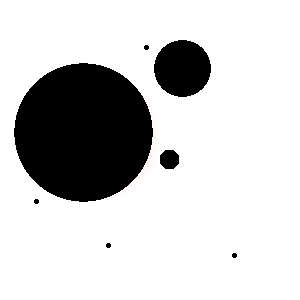
\includegraphics[height=3cm]{Images/gaussian_spilling_init.png}
  
\includegraphics[height=3cm]{Images/gaussian_spilling_g10.png}
  
\includegraphics[height=3cm]{Images/gaussian_spilling_g40.png}
  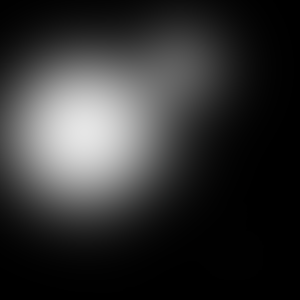
\includegraphics[height=3cm]{Images/gaussian_spilling_g100.png}
  \label{fig:scale_space_spilling}
  \caption{débordement du signal des structures larges sur les structures de plus petite tailles}
\end{figure}

\begin{figure}
  \centering
  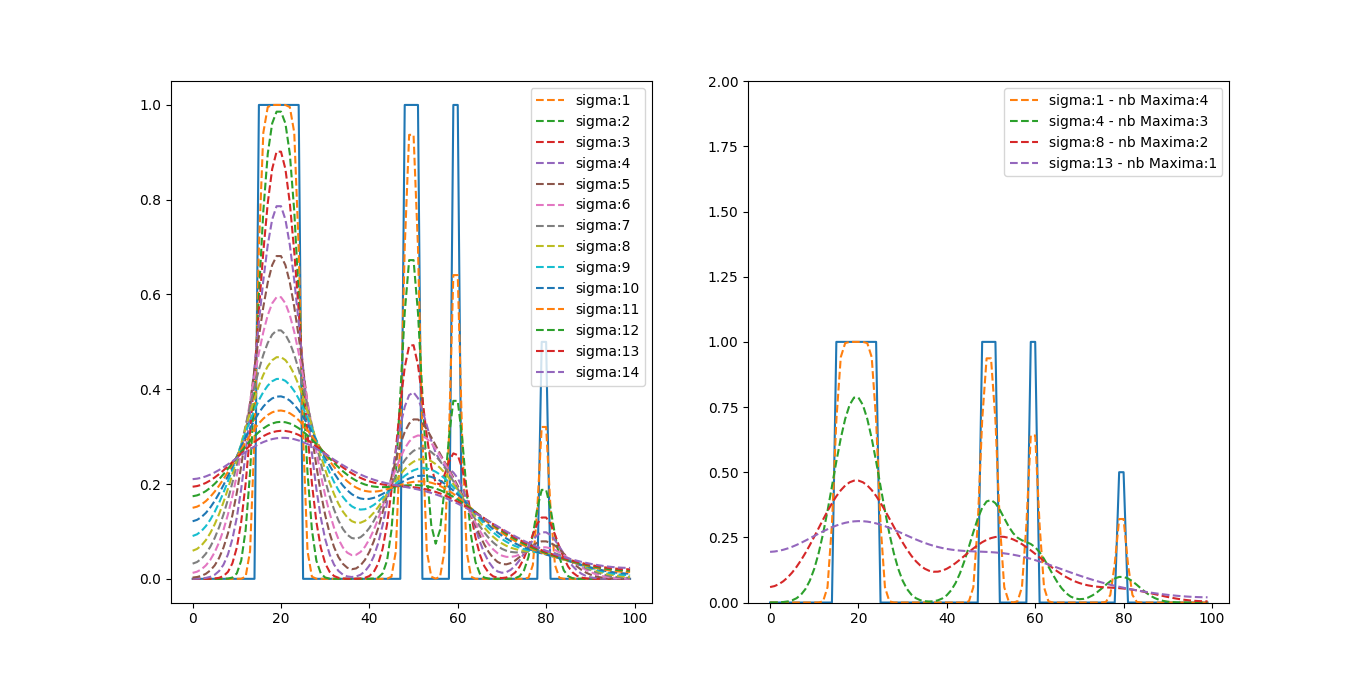
\includegraphics[height=5cm]{Images/GSP_experiment.png}
  \label{fig:scale_space_spilling2}
  \caption{Effet du lissage sur les structures en fonction de $\sigma$. Deux phénomènes sont observés, la fusion et le déplacement des pics des structures adjacentes. Le lissage fait disparaître les structures de faible intensité ou trop fines.}
\end{figure}



\subsection{granulométrie}
\label{sec:EA:rehaussement:echelle:granulometrie}

La granulométrie est l'étude des tailles des particules d'un échantillon. En chimie, on utilise par exemple la technique du tamisage. Elle permet, grâce à un tamis et une grille dont on contrôle la taille du maillage, de ne conserver que des particules dont la taille est trop grosse pour passer à travers le tamis.

Un principe similaire est applicable en morphologie mathématique sur les images binaires et par extension en niveau de gris.

\subsubsection{Érosion et dilatation }

Deux opérations élémentaire, la dilatation et l'érosion, permettent de définir les opérations nécessaires pour définir un espace d'échelle morphologique. Les définitions qui vont suivre sont des opérations binaires relatives à des objets blancs sur fond noir.

\paragraph{Définitions}
% definition de Digital image processing, Gonzalez second edition, Mophology - p518
Soit deux ensembles définis dans $Z^3$ avec les composants $a=(a_1,a_2,a_3)$ et $b=(b_1,b_2,b_3)$.

La \emph{translation} de $A$ par $x = (x_1,x_2)$, noté $(A)_x$ est définie par :
% étrange cette formulation c|c non défini, idem pour x|x dans les autres.
\begin{equation}
  (A)_x = \{c|c = a+x, pour a \in A\}. 
\end{equation}

On définit la \emph{réflection} de B, dénoté $\widehat{B}$ par :

\begin{equation}
  (\widehat{B}) = \{x|x = -b, pour b \in B\}. 
\end{equation}

Le complémentaire de l'ensemble $A$ est défini par :

\begin{equation}
  (A^c) = \{x|x \not\in A\}. 
\end{equation}

La différence de deux ensemble $A$ et $B$, noté $A - B$, est défini par:

\begin{equation}
  (A-B) = \{x|x \in A, x\not\in \} = A \cap B^c.  
\end{equation}


\paragraph{dilatation}
En utilisant les propriétés précédentes, la dilatation s'exprime de la manière suivante :

\begin{equation}
 A \oplus B = {x|(\widehat{B}_x, \cap A \neq = \emptyset }
\end{equation}

La dilatation de $A$ par $B$ est l'ensemble de tous les déplacements de $\widehat{B}$ tel qu'il y ai au moins un pixel de recouvrement entre $A$ et $\widehat{B}$. Cette opération permet de faire grossir une structure en fonction de la forme de B.

\begin{figure}
  \centering
  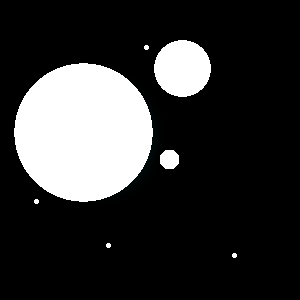
\includegraphics[height=3cm]{Images/morpho_init.png}
  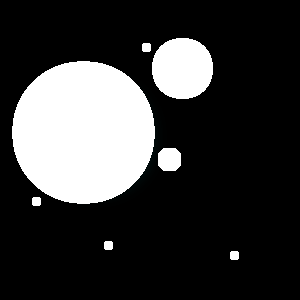
\includegraphics[height=3cm]{Images/morpho_dilate_k5.png}
  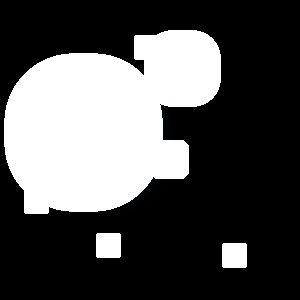
\includegraphics[height=3cm]{Images/morpho_dilate_k21.png}
  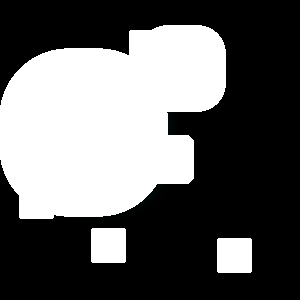
\includegraphics[height=3cm]{Images/morpho_dilate_k31.png}
  \label{fig:morpho_dilation}
  \caption{Exemple de dilatation}
\end{figure}

L'ensemble $B$ est couramment appelé \emph{élément structurant}.

\paragraph{érosion}

L'opération opposée à la dilatation est l'érosion.

\begin{equation}
  A \ominus B = {x|(B)_x, \subseteq A}
\end{equation}

L'érosion de $A$ par $B$ est l'ensemble de tous les points $x$ tel que $B$ translaté de x est inclus dans $A$. 

\begin{figure}
  \centering
  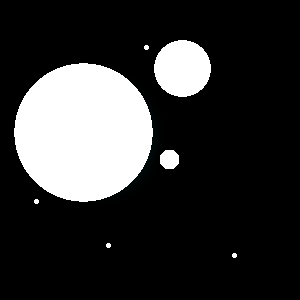
\includegraphics[height=3cm]{Images/morpho_init.png}
  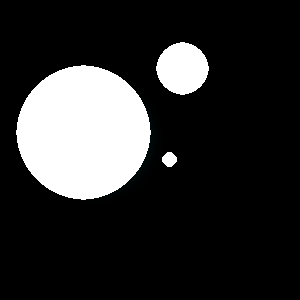
\includegraphics[height=3cm]{Images/morpho_erode_k5.png}
  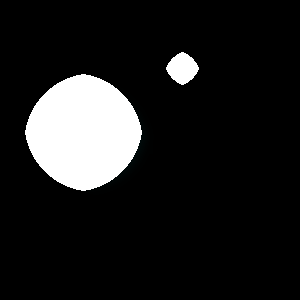
\includegraphics[height=3cm]{Images/morpho_erode_k21.png}
  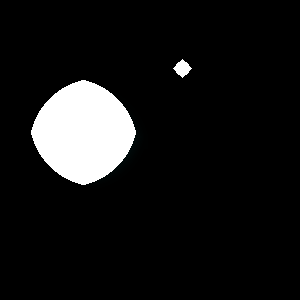
\includegraphics[height=3cm]{Images/morpho_erode_k31.png}
  \label{fig:morpho_erosion}
  \caption{Exemple d'érosion}
\end{figure}

\subsubsection{Fermeture et ouverture}

A partir des opérations d'érosion et de dilatation, on peut définir des opération composites, l'ouverture et la fermeture.

\paragraph{Fermeture}
L'ouverture est définie comme la dilatation de $A$ par $B$ suivi de l'érosion de $A$ par $B$.
\begin{equation}
 A \bullet B = (A \oplus B) \ominus B
\end{equation}

Cet opérateur est utilisé pour boucher les trous dont la surface est inférieure à la surface de l'élément structurant. L'érosion qui suit la dilatation permet d'assurer que la taille reste stable.

\begin{figure}
  \centering
  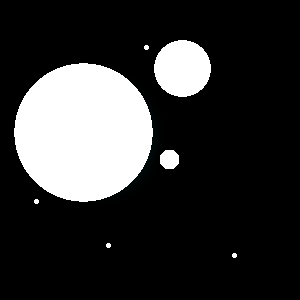
\includegraphics[height=3cm]{Images/morpho_init.png}
  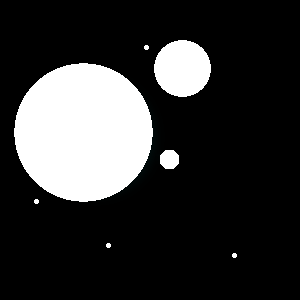
\includegraphics[height=3cm]{Images/morpho_close_k5.png}
  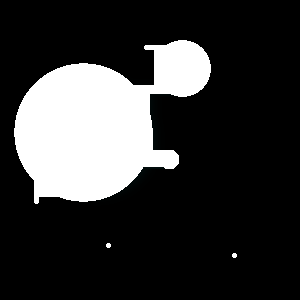
\includegraphics[height=3cm]{Images/morpho_close_k21.png}
  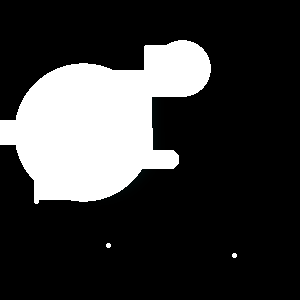
\includegraphics[height=3cm]{Images/morpho_close_k31.png}
  \label{fig:morpho_femerture}
  \caption{Exemple de fermeture}
\end{figure}

\paragraph{Ouverture}
L'ouverture est définie comme l'érosion de $A$ par $B$ suivi de la dilatation de $A$ par $B$.
\begin{equation}
 A \circ B = (A \ominus B) \oplus B
\end{equation}

\begin{figure}
  \centering
  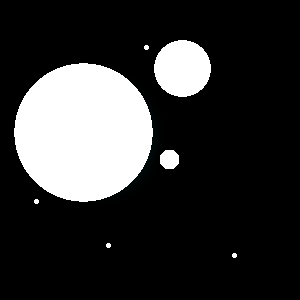
\includegraphics[height=3cm]{Images/morpho_init.png}
  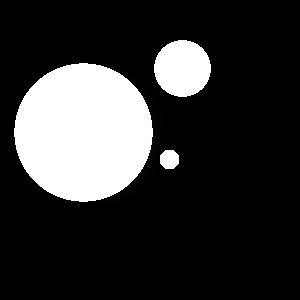
\includegraphics[height=3cm]{Images/morpho_open_k5.png}
  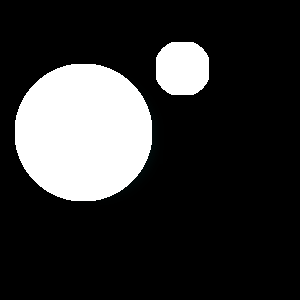
\includegraphics[height=3cm]{Images/morpho_open_k21.png}
  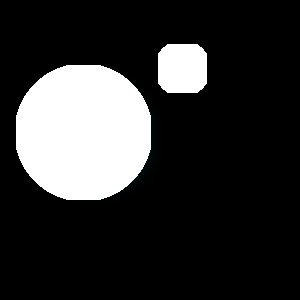
\includegraphics[height=3cm]{Images/morpho_open_k31.png}
  \label{fig:morpho_ouverture}
  \caption{Exemple d'ouverture}
\end{figure}

Cet opérateur est utilisé pour supprimer les structures de tailles inférieures à la surface de l'élément structurant. La dilatation qui suit l'érosion permet d'assurer que la taille des éléments restent stable.

L'ouverture permet de construire un espace d'échelle paramétré par la taille de l'élément structurant. Cet espace ne souffre pas d'une fusion parasite des structures adjacentes.

\subsection{Flux}
\label{sec:EA:rehaussement:echelle:flux}

Comme nous l'avons vu dans la section SEC. \ref{sec:EA:rehaussement:echelle:gaussien}, l'espace d'échelle gaussien peut provoquer des débordements de structures sur d'autres, plus petites. On peut limiter se problème en utilisant un cadre différent, celui de l'analyse des flux.

Si l'on considère un champ de vecteur $V$, par exemple un fluide, ou un champ de gradient pour une image, on défini le flux passant à travers la surface $S$ orienté par sa normale $\vec{n_s}$ comme l'intégrale de la somme du produit scalaire entre le vecteur de flux $\vec{v}$ et la normale à la surface $\vec{n}$.

\begin{equation}
flux_S = \int_{S}< \vec{v},\vec{n} > d\rho
\end{equation}

On peut appliquer le calcul de flux à la surface d'un objet fermé. En particulier, des structures en forme de disques ou de sphères ont été particulièrement utilisées pour l'analyse de vaisseaux sanguins. On peut en effet contrôler directement le diamètre d'une sphère pour détecter les objets de la taille voulue. Cette formulation de l'échelle diffère des méthodes précédentes, car les objets tubulaires ne sont détectés que pour une échelle donnée, là ou les deux autres techniques conservent les objets à l'échelle donnée et aux échelles supérieures. Elle a aussi l'avantage de limiter l'analyse du flux à la surface de la sphère et donc de produire une réponse qui ne déborde pas.

La précision du calcul de l'intégrale de flux dépend du nombre d'échantillonages effectués sur $S$. Plus celui-ci est grand, plus le calcul est coûteux. De plus, plus l'échelle sélectionnée est grande, et donc plus la surface de la sphère est grande, plus le nombre d'échantillonage requis est important.

Law propose une formulation élégante du calcul de flux dans le domaine de Fourier afin de réduire drastiquement le temps de calcul par rapport à l'implémentation naïve \cite{Law2009_efficient_implementation}.

Pour y parvenir, Law propose d'exprimer le calcul de flux sous la forme d'une convolution dans le domaine temporel. L'avantage de la convolution est double, on évite l'étape d'échantillonage sur la surface et la convolution s'exprime comme une multiplication dans le domaine de Fourier. On peut exprimer le calcul de flux en terme de volume et non plus en terme de surface grâce au théorème de la divergence qui établit une égalité entre le flux à la surface d'un objet et le flux à l'intérieur de son volume. Ainsi :

\begin{equation}
  flux_{\partial C} = \int_{\partial C}< \vec{v},\vec{n} > d\rho \equiv \int_{C }\Delta I d\nu
\end{equation}

Plus précisément :

\begin{equation}
  f_s(x,y,z) = \int_{R_s}\vec{v}(x+t,y+p, z+q) . \vec{n}_{(t,p,q)}dA
\end{equation}

avec $R_s$ une région sphérique de rayon $s$; $dA$ une surface infinitésimale sur la surface $\partial R_s$; $\vec{n}_{(t,p,q)}dA$ le vecteur normal à $dA$ à la position $(t,p,q)$; et $\vec{v}$ le gradient de l'image $I$. $\vec{v}$ est obtenu à partir de l'image $I$ lissée par un noyau Gaussien afin d'assurer la dérivabilité du signal de $I$. $\vec{v}=\nabla(g*I)$.

Qui est équivalent à :

\begin{align}
  f_s(x,y,z) & = \int_{R_s} \vec{div}( \vec{v}(x+t,y+p, z+q) ) dtdpdq \\
  & = \int_{\omega} d_s(t,p,q) [\vec{div}( \vec{v}(x+t,y+p, z+q) )] dtdpdq
\end{align}

où $\omega$ est le domaine entier de l'image et $d_s(t,p,q)$ correspond à la fonction porte sphérique définie par :

\begin{equation}
d_s(x,y,z) = [\sqrt{x^2 + y^2 + z^2} \leq s]
\end{equation}

Ainsi, $f_s(x,y,z)$ peut être exprimé sous forme de convolution :
\begin{align}
  f_s(x,y,z) & = \int_{\omega} d_s(t,p,q) [\vec{div}( \vec{v}(x+t,y+p, z+q) )] dtdpdq \\
             & = \int_{\omega} d_s(t,p,q) (\Delta(g*I(x+t,y+p, z+q)))] dtdpdq \\
             & = \int_{\omega} d_s(-t,-p,-q) (\Delta(g*I(x+t,y+p, z+q)))] dtdpdq \\
             & = d_s * \Delta g * I(x,y,z) \\
             & = I * h_s(x,y,z) \\
\end{align}

avec $*$ l'opérateur de convolution, $\Delta$ l'opérateur laplacien.

Et dans le domaine de Fourier:

\begin{align}
  FFT( I * h_s(x,y,z) ) &= FFT(I) . H_s(u,v,w) \\
                       &= FFT(I) . [ (j2 \pi)^2 ( (\frac{u}{N_x})^2 + (\frac{v}{N_y})^2 + (\frac{w}{N_z})^2 ) ] \\
                       & . [ exp( -( (\frac{u}{N_x})^2 + (\frac{v}{N_y})^2 + (\frac{w}{N_z})^2 ) 2(\pi\sigma)^2 ) ]
\end{align}

\begin{figure}
  \centering
  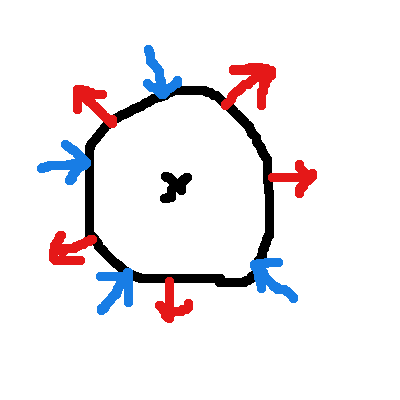
\includegraphics[height=6cm]{Images/flux.png}
  \label{fig:flux_sphere}
  \caption{flux sur la surface d'une sphère}
\end{figure}

\subsection{Multi-échelle}
\label{sec:EA:rehaussement:echelle:multiScale}

\todo{Voir si cette partie est à développer, ou simplement à mentionner}

La combinaison de la détection de vaisseaux à plusieurs échelles est principalement fusionné grâce à un opérateur max effectué sur toutes les échelles.

\begin{equation}
  V(I)_{multi echelle} = max_{\sigma}V_{\sigma}(I)
\end{equation}

Cet opérateur peut provoquer un recouvrement des structures adjacentes par une structure ayant une réponse plus haute. A notre connaissance, aucune publication ne propose de pondérer ou de hiérachiser la réponse en fonction de la taille du $\sigma$ (i.e. la taille des vaisseaux).

\section{Familles de rehaussement}
\label{sec:EA:rehaussement:famille}

Plusieurs grandes familles de rehaussement sont présentes dans la littérature. 

\subsection{Morphologie}
\label{sec:EA:rehaussement:morpho}

Le rehaussement à base d'opérateurs morphologiques s'articule autour de deux familles, la composition d'éléments structurants rigides et l'utilisation de chemins curvilinéaires flexibles.

La composition d'éléments structurants rigides s'effectue la plupart du temps avec des boules et des cylindres. Les cylindres permettent de couvrir les parties curvilignes des vaisseaux, tandis que les boules couvrent les jonctions. Une composition d'ouvertures avec ces éléments est ensuite utilisée pour récupérer le réseau vasculaire. Sazak propose une schéma de ce type en 2 dimensions \cite{Sazak2019_bowler_hat_2D} puis en 3D \cite{Sazak2018_bowler_hat_3D} et compare son efficacité contre du rehaussement à base de tenseurs de phases et hessiens. Cette méthode bien que simple à mettre en pratique, nécessite plusieurs itérations avec des rotations des éléments structurants afin de capturer toutes les orientations des structures tubulaires. Cette méthode peut devenir coûteuse en 3D.

\begin{figure}
  \centering
  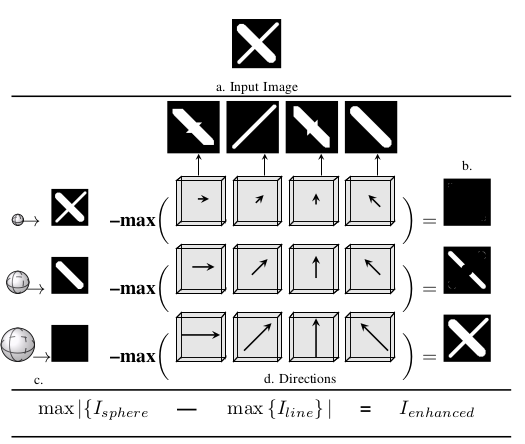
\includegraphics[height=4cm]{Images/bowlerHat_3D.png}
  \label{fig:sazak_bowler_hat}
  \caption{bowler hat transform proposée par Sazak et al. La combinaison d'éléments sphériques et linéaires permet de capture les structures curvilinéaires. }
\end{figure}

L'un des défaut de la méthode précédente est la rigidité des éléments structurants qui ne permettent pas toujours de capturer les variations de formes des vaisseaux. Hejimans \cite{Heijmans2005_path_opening} propose une famille d'éléments structurants flexibles dont la forme est définie par une grille d'adjacences. Des améliorations successives de cet algorithme ont été proposés : XX propose une implémentation efficace de l'agorithm en O(XX), Cokelaer propose une version robuste au bruit en autorisant des discontinuités dans l'élément structurant, Merveille et al. itère en proposant un classement de l'orientation des chemins afin de segmenter les vaisseaux dans des images 2D et 3D.

\subsection{Phase}
\label{sec:EA:rehaussement:Phase}

Une image peut-être à la fois vue comme une matrice de pixels et comme un signal discret en 2 ou 3 dimensions. Lorsque l'on considère la représentation sous forme de signal on peut décomposer celui-ci en deux éléments indépendants : L'amplitude, correspondant à l'intensité des pixels et la phase, correspondant à la distance entre deux pics de deux signaux. La phase étant une mesure relative à la position des pics, elle ne prend pas en compte l'amplitude de ceux-ci et présente donc une invariance aux changements d'intensités. Oppenhei et al. \cite{Oppenheim1981_phase_importance} démontre l'importance de ces caractéristiques de l'image et montre une correspondance avec le système visuel humain. 

\begin{figure}
  \centering
  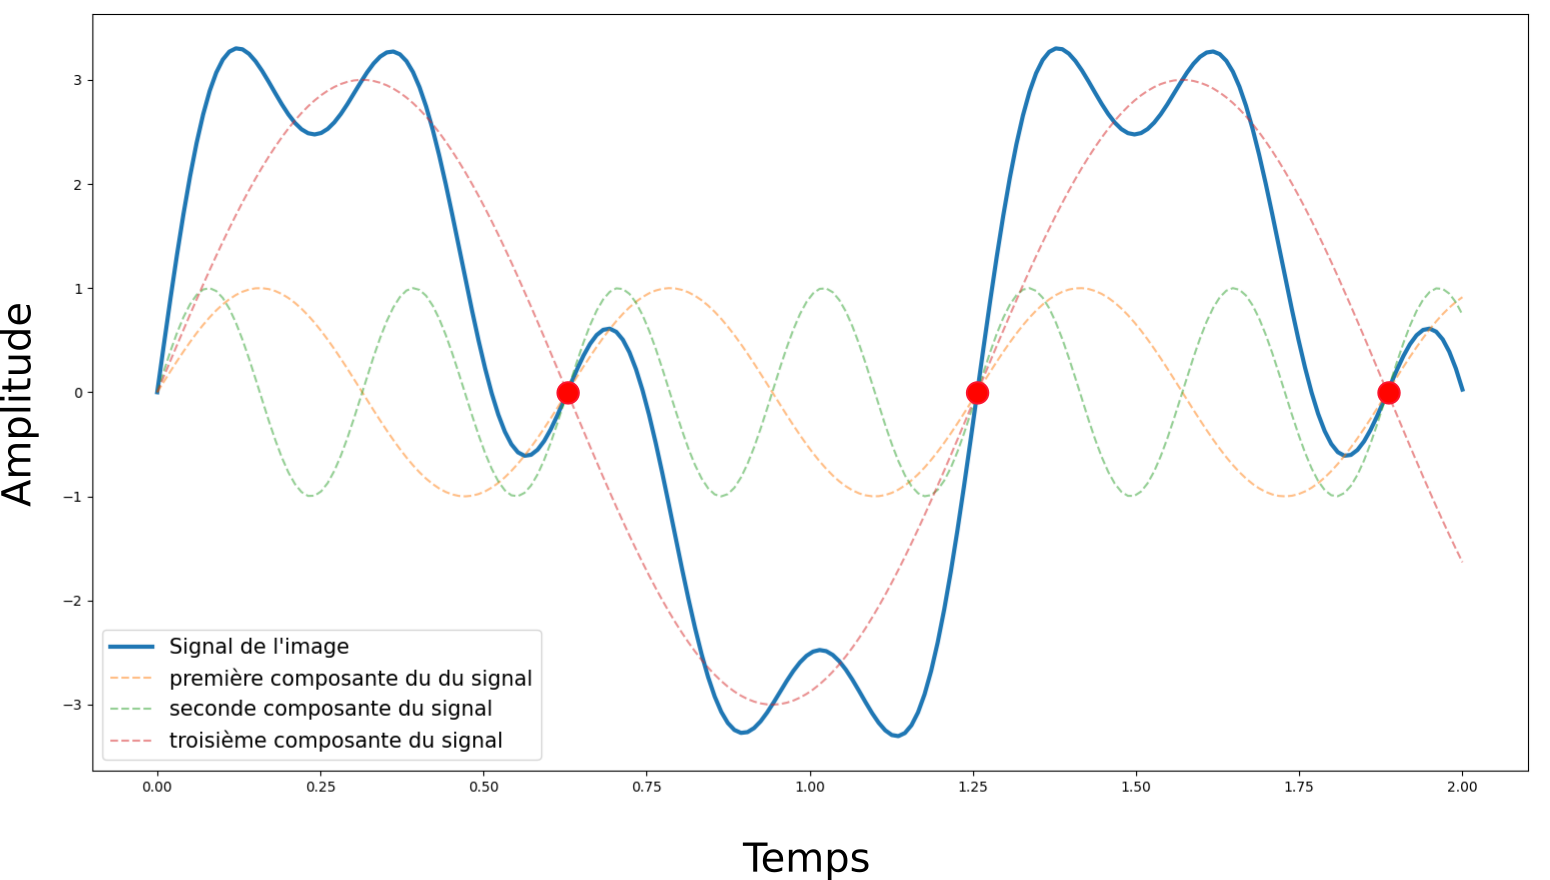
\includegraphics[height=5cm]{Images/PC_decomposition.png}
  \label{fig:phase congruency}
  \caption{Décomposition de Fourier d'un signal, en certains points la phase de chaque composant est synchronisée}
\end{figure}

Plusieurs structures de vesselness se basent sur cette propriété pour la détection des vaisseaux. Obara et al. \cite{Obara2012_phase} utilise un tenseur de structure basé sur le contraste de phase. Les valeurs propres de ce tenseur permettent ensuite d'exprimer une mesure de tubularité.

Ce tenseur est exprimé comme :

\begin{equation}
  T_{PC} = \sum PC_{o}(p)(n_{o}n^T - \alpha \text{I})
\end{equation}

Avec $PC(x)$ la fonction de congruence de phase, $n(\theta)=[cos(\theta),sin(\theta)]^T$ le vecteur d'orientation $o$,$\alpha = 1/(m-1)$ et $I$ le tenseur unitaire. $PC(x)$ permet de détecter les éléments saillants à la manière d'un détecteur de contours.
En effet, une image vue comme un signal peut être décomposée comme un ensemble de signaux sinusoïdaux. Les éléments saillants tel que les bordures ou les coins d'objets correspondent à une synchronisation, e.g congruence, de ces signaux pour un angle donné. Celle-ci s'exprime par :

\begin{equation}
  PC(x) = max_{\theta \in [0,2\pi)} \sum  \frac{ \alpha_{\omega}cos(\omega x + \phi_{\omega} - \omega)  }{ \alpha_{\omega}d \omega } d \omega
\end{equation}

Celle-ci représente la variance de phase des différents signaux au point $x$. Lorsque les phases des signaux sont égales $PC(x)=1$.
En pratique, cette définition est complexe à implémenter, on lui préfère en pratique la mesure d'énergie locale qui s'approxime avec des filtres de Gabor ou des ondelettes. Ces filtres sont basés sur des gaussiennes dont on peut contrôler l'échelle comme un espace gaussien.

\begin{figure}
  \centering
  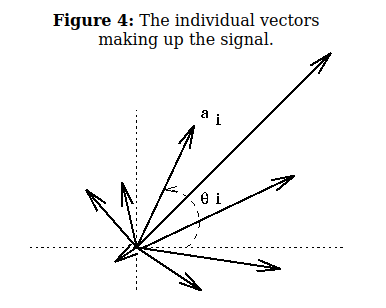
\includegraphics[height=5cm]{Images/PC_vectors.png}
  \label{fig:phase congruency}
  \caption{représentation vectorielle d'un signal, chaque vecteur représente une composante sinusoïdale paramétrée par sa phase pour l'orientation et son amplitude pour sa norme}
\end{figure}

Enfin, ces filtres sont dépendants du nombre d'orientations échantillonnées $\omega$. En pratique entre 6 et 10 échantillons régulièrement espacés suffisent. 

\subsection{Hessienne}
\label{sec:EA:rehaussement:hessienne}

La matrice hessienne est la matrice des dérivées seconde de l'image en un pixel. Celle-ci permet d'exprimer la courbure locale autour d'un point.
Les valeurs propres et vecteurs propres de la hessienne permettent de quantifier l'orientation, le sens et l'amplitude du voisinage d'un point.
La simplicité de la Hessienne a permis l'émergence de nombreuses modélisations de rehaussement.

En 3D, une structure tubulaire parfaite peut-être exprimée par les valeurs propres. Soit $\lambda_1$,$\lambda_2$,$\lambda_3$ tel que $|\lambda_1| \leq |\lambda_2| \leq |\lambda_3|$ alors un tube parfait est modélisée par :

\begin{align}
  \lambda_1 \approx 0 \\
  \lambda_1 \ll \lambda_2 \\
  \lambda_2 \approx \lambda_3
\end{align}

Ces équations sont valables dans un contexte spécifique. Lorsque le $\sigma$ de l'espace d'échelle coïncide avec la taille d'une structure tubulaire, la ligne centrale de celle-ci devient un maxima local. Le vecteur propre $\lambda_1 \approx 0$ correspond à la direction du tube. Dans ce cas, la magnitude $\lambda_1$ est proche de zéro car le gradient dans cette direction est presque nul. Dans les deux directions principales de la tranche, l'intensité du tube décroissant rapidement au fur et à mesure que l'on s'éloigne du centre, les valeurs propres $\lambda_2$ et $\lambda_3$ sont donc élevées.

Cet outils a permis le développement de nombreuses techniques de rehaussement basé sur les valeurs propres tel que Li et al. \cite{Li2003_vesselness}, Erdt et al. \cite{Erdt2008_liver_vesselness}, Frangi et al. \cite{Frangi1998_vesselness}, Sato et al. \cite{Sato1998_vesselness}, Jerman et al. \cite{Jerman2015_beyond_frangi}, Meijering et al. \cite{Meijering2004_neurite_vesselness}, etc. dont les principales contributions sont présentées dans le chapitre SEC. \ref{sec:Bench:filtres}.

\subsection{Diffusion}
\label{sec:EA:rehaussement:diffusion}

Les méthodes de diffusions sont une classe un peu à part dans le rehaussement des vaisseaux. L'objectif des frameworks de diffusion est d'améliorer le signal des vaisseaux en homogénéisant leur intensités et en renforçant leurs bordures. Pour cela, les filtres de diffusion proposent un schéma de lissage itératif qui prennent en compte la géométrie des structures à lisser.

HDCS \cite{Mendrik2009_HDCS} (Hybrid diffusion with continuous switch), propose un lissage hybride combinant lissage isotropique de régions et lissage basé sur les bordures. Ces deux lissages sont combinés avec une mesure de la géométrie locale afin d'appliquer une combinaison linéaire des deux filtres la plus adaptée.

VED \cite{Manniesing2006_VED} (Vessel enhancement diffusion)propose un lissage basé sur les méthodes de rehaussement hessiens. Ce cadre permet ainsi d'homogénéiser la réponse de n'importe quelle filtre de rehaussement hessien sans perdre de structures tubulaires.

Ces méthodes itératives sont coûteuses en temps de calcul et nécessitent une paramétrisation supplémentaire pour contrôler la force du lissage ainsi que le nombre d'itérations nécessaire.

\section{Bilan et orientation des travaux}
\label{sec:EA:bilan}

Les constatations émises après l'état de l'art de la segmentation sont sensiblement les mêmes pour le rehaussement de vaisseaux. Les articles originaux testent souvent leurs méthodes sur des structures synthétiques simples ou des exemples variés. Elles sont toujours testés contre 2 à 4 autres méthodes. Lorsqu'ils sont utilisés sur des données réelles, les filtres de rehaussement sont largement utilisés avec les paramètres recommandés par l'auteur, sans adaptation à une application particulière.

Quelques travaux portent sur la comparaison des filtres de rehaussement. Luu et al. \cite{Luu2015_liver_vesselness_comparison} propose une comparaison de 3 filtres de rehaussement et 3 filtres de diffusion pour la tomodensitométrie du foie. Phellan et al. \cite{Phellan2017_Brain_vesselness_comparison} propose une comparaison de 6 filtres de rehaussement et 3 filtres de diffusions pour l'IRM du cerveau et un jeu de données synthétique.

Cependant ces travaux ne nous permettent pas de répondre à plusieurs questions :

\begin{itemize}
\item Quel filtre utiliser pour l'IRM du foie ?
\item Quel est l'impacte de la paramétrisation sur la réponse des filtres ?
\item Quels types de vaisseaux sont le mieux rehaussés ?
\item Quel est l'impacte des filtres de rehaussement indépendamment de la segmentation ?
\end{itemize}
